\documentclass[a4paper,10pt]{article}
\usepackage[hidelinks]{hyperref}
\usepackage{float}
\usepackage{graphicx}
\usepackage{listings}
\usepackage[utf8]{inputenc}

%%% Title
\title{Processo e Sviluppo Software: Assignment 3} 
\author{Ivo Junior Bettini - 806878, Umberto Cocca - 807191, \\Silvia Traversa - 816435\\
\href{https://gitlab.com/s.traversa/2019_assignment3_booksloan}{GitLab repository}}
\date{}

\begin{document}

\maketitle 

\section*{Applicazione}
L'applicazione BooksLoan permette agli utenti di visualizzare il catalogo di una biblioteca. Essi possono visualizzare sia le copie disponibili e non, dei libri ed eventualmente richiederne una in prestito.
È inoltre possibile visualizzare le informazioni relative a ogni singolo libro, quali l'autore o la presenza di sequel.\\ 

\noindent Gli amministratori, che si dividono in amministratori con contratto a tempo indeterminato e amministratori con contratto a tempo determinato, differiscono per la possibilità di eliminare i libri. Possono entrambi interagire con un'area CMS eseguendo il CRUD delle principali entità. Questa differenziazione di operatività nasce con l'idea di dare maggior responsabilità e controllo.

\section*{Esecuzione dell'applicazione}
\subsection*{Preparazione Database}
Prima di eseguire l'applicazione, è necessario importare i dati e la struttura del database, creato con MySQL.\\\\
Per effettuare questa operazione bisogna effettuare su MySQLWorkbench un Data Import del file \textit{DumpFinale} presente nella cartella \textit{dumps}. Successivamente, per permettere la connessione al database, è richiesta la modifica del file \textit{src/main/resources/application.properties} inserendo le proprie credenziali MySQL nei campi spring.datasource.username e spring.datasource.password, come illustrato nella figura.\\
\begin{figure}[H]
	\centering
	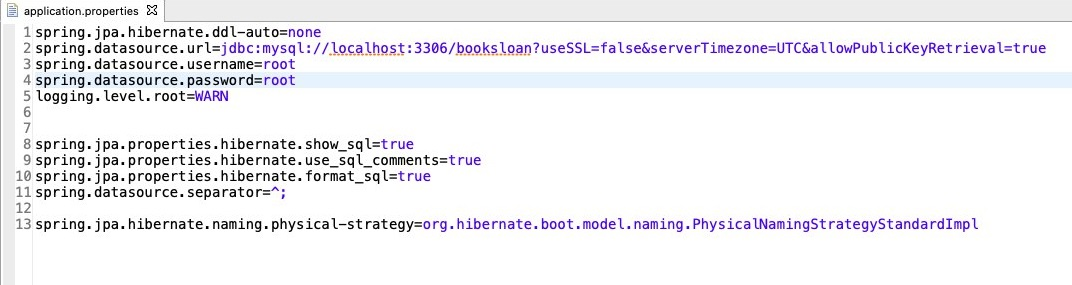
\includegraphics[width=1\linewidth]{images/properties}
\end{figure}
\newpage

\subsection*{Avvio Applicazione}

Per far partire l'applicazione, dopo aver clonato il repository, eseguire le seguenti righe di comando:\\

\begin{lstlisting}[language=bash]
	mvnw clean package spring-boot:repackage
\end{lstlisting}

\begin{lstlisting}[language=bash]
	java target/BooksLoan-1.jar
\end{lstlisting}

\noindent \\L'applicazione sarà disponibile all'indirizzo \href{http://localhost:8080}{http://localhost:8080}.\\

\noindent Per accedere alle funzionalità dell'applicazione è rischiesto un login, che è possibile effettuare con tre tipi diversi di account, rappresentativi di categorie:

\begin{itemize}
	\item \textbf{amministratore con contratto a tempo indeterminato:}
\begin{lstlisting}[language=bash]
    username: 123 password: 1234
\end{lstlisting}
	\item \textbf{amministratore con contratto a tempo determinato:}
\begin{lstlisting}[language=bash]
    username: 456 password: 4567
\end{lstlisting}
	\item \textbf{cliente:}
\begin{lstlisting}[language=bash]
    username: 321 password: 1234
\end{lstlisting}
\end{itemize}

\section*{Schema E-R}

\begin{figure}[H]
	\centering
	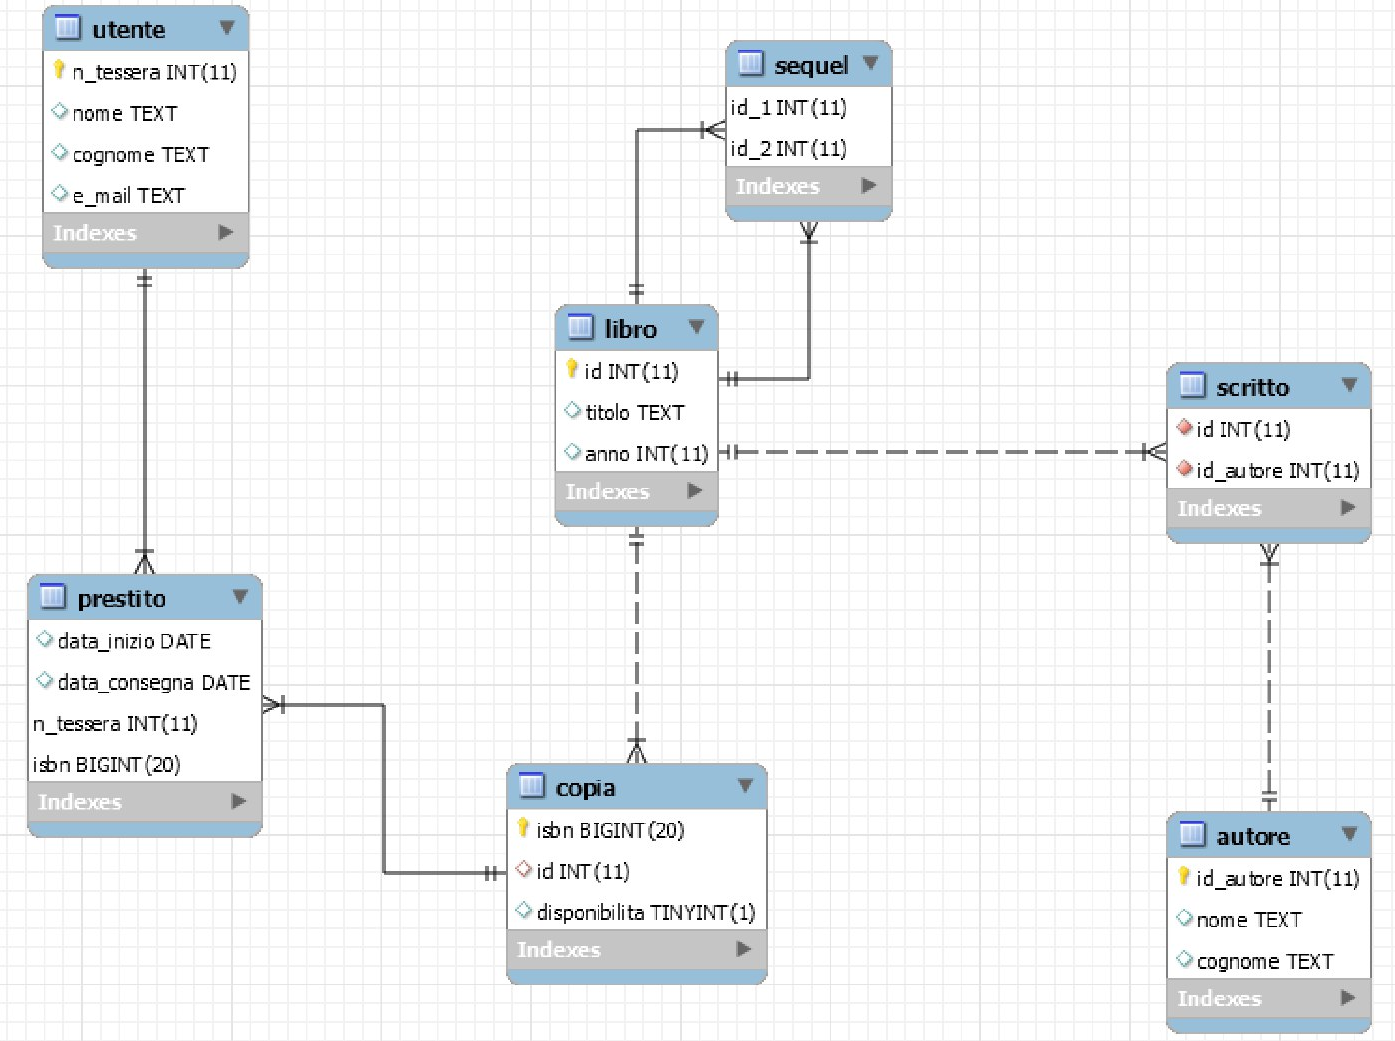
\includegraphics[width=0.8\linewidth]{images/ERdiagram}
	\caption[Schema ER]{Schema ER}
	\label{fig:re}
\end{figure}

Le entità utilizzate nel nostro progetto sono così descritte:

\begin{itemize}
	\item Utente: descrive la persona registrata e che utilizza il sito. Gli attributi n\_tessera e password rappresentano le credenziali d'accesso al sito, mentre l'attributo ruolo determina se l'utente è un amministratore o un utente.
	\item Libro: elemento che compone la nostra libreria online.
	\item Copia: insieme di diverse edizioni di un libro che possiedono l'ISBN come chiave primaria. Una copia può trovarsi in due stati, disponibile o non disponibile (in quest'ultimo caso non può essere presa in prestito).
	\item Autore: colui che ha scritto uno o più libri.
\end{itemize}

Esse sono messe in relazione da:
\begin{itemize}
	\item Prestito: entità che relaziona utente con copia. Un utente può prenotare più copie dello stesso libro.
	\item Sequel: entità che mette in relazione un libro con se stesso. Un libro può possedere zero o più sequel (nell'applicazione rendiamo visibile solo il diretto successivo).
	\item Scritto: entità che mette in relazione autore con libro. Un libro può essere scritto da più autori e un autore può scrivere più libri.
\end{itemize}

\section*{Pattern MVC}
Ai fini del progetto si è utilizzato il pattern architetturale Model-view-controller (MVC), per separare la logica di presentazione dei dati dalla logica di business.\\

\sloppy\noindent Il package \textbf{net.assignment.booksLoan.model} contiene al suo interno l'implementazione delle classi presenti nello \textit{Schema E-R}. Sono state annotate le classi e i rispettivi membri con le annotazioni della Java Persistance API (JPA), un framework che nasce per garantire la persistenza dei dati.\\

\noindent Per mezzo del Controller viene implementata la logica di controllo dell'applicazione. All'interno delle classi Controller vengono eseguiti i metodi per gestire le richieste Get e Post dell'utente reperendo le informazioni attraverso i layer repository che permettono di dare un'ulteriore livello di astrazione sull'accesso dei dati, potendo eseguire il CRUD, e grazie ai layer service che espongono la logica di business ottenendo così i Model da mostrare in View.

\section*{BooksLoan}
Per poter accedere all’applicazione bisogna obbligatoriamente essere registrati. Attraverso l'utilizzo della dipendenza Spring Security viene controllato l'accesso, impedendone la navigazione tra le pagine se non si è registrati e gestendone i livelli d'accesso. Nello specifico un cliente non può accedere alle pagine di un amministratore.\\

\noindent Abbiamo deciso di distinguere l'amministratore in due divere tipologie, che si differenziano in base al loro tipo di contratto. Questa scelta è stata fatta pensando all'organizzazione interna di una biblioteca, e anche perchè in questo modo abbiamo creato diversi livelli di privilegi e di operazioni eseguibili da un utente. 
L'amministratore con un contratto a tempo indeterminato, una volta che ha eseguito il login, ha la possibilità di effettuare ogni tipo di operazione: può eliminare, aggiungere, modificare libri e impostare le copie, gli autori e i sequel di un libro.
Un amministratore con contratto a tempo determinato, invece, non può cancellare i libri e le sue relative copie.\\

\noindent Il cliente, una volta effettuato il login, ha a disposizione l'elenco dei libri del catalogo della biblioteca. Questi sono riportati in una tabella in cui è possibile filtrare cercando per chiave. Il filtraggio è stato eseguito utilizzando jQuery. Inoltre, il cliente può visualizzare se è presente una copia disponibile di un determinato libro ed eventualmente prenderla in prestito, può visualizzare i suoi prestiti in corso e restituire una copia. La restituzione rende disponibile la copia stessa e quindi accessibile da altri clienti per la prenotazione.\\

\end{document}